Implementada a solução final, foram testadas várias configurações
que permitissem demonstrar o poder do motor desenvolvido,
utilizando luzes, texturas, animações, etc...//
//
As cenas seguintes representam, então, as imagens criadas pelas
configurações dadas, que de certa forma refletem a capacidade
final do motor desenvolvido. Estas podem ser observadas em
\ref{fig:teapot}, \ref{fig:sisolar1}.

\subsection{Boneco de neve}

\begin{center}
    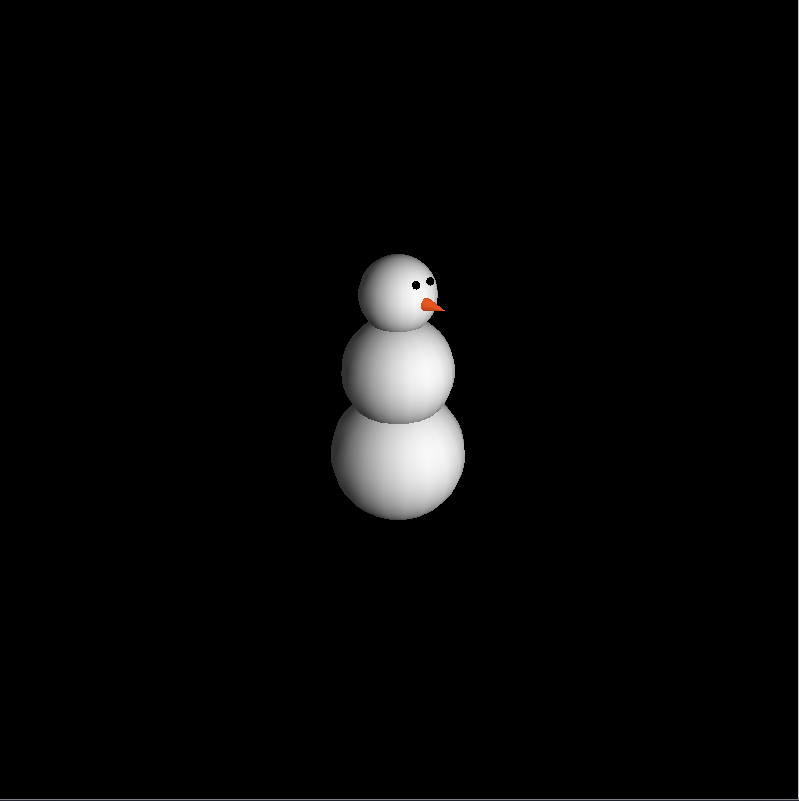
\includegraphics[width=0.8\textwidth]{imgs/boneco.png}
    \captionof{figure}{Boneco de neve}
    \label{fig:teapot}
\end{center}

\subsection{Rua com cone}

\begin{center}
    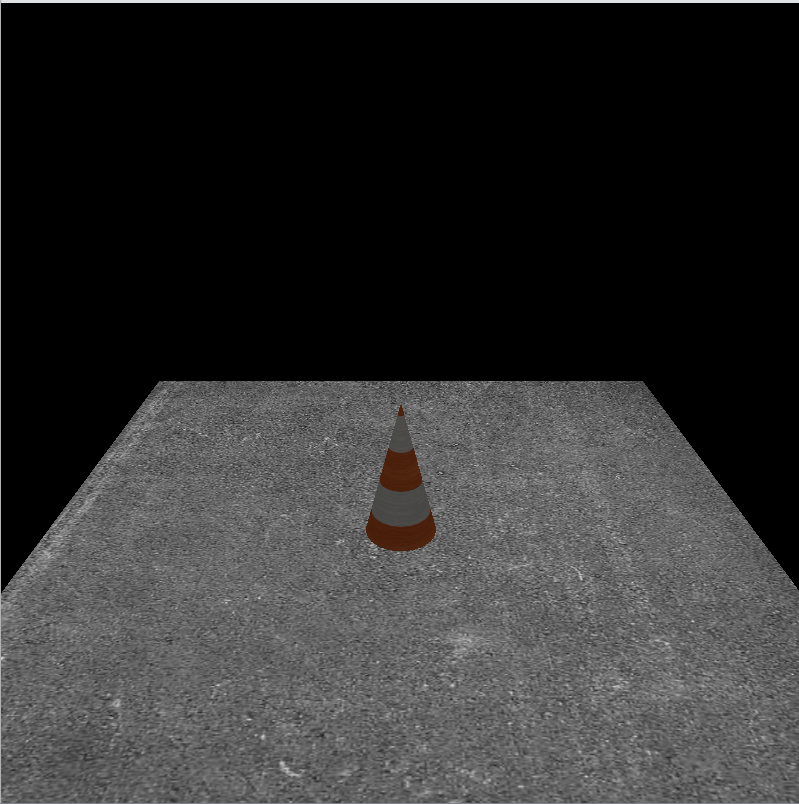
\includegraphics[width=0.8\textwidth]{imgs/capa.png}
    \captionof{figure}{Rua com cone}
    \label{fig:sisolar1}
\end{center}

